% \textbf{\underline{OZ 4 - De wet van Ampère en de wet van Biot-Savart - Oefening 2:}}
% \vspace{0.5cm}

% Bepaal de grootte en de richting van het magnetisch veld dat gegenereerd wordt in punt $ P $ als een stroom $ I $ door de draad in Figuur 4.2 wordt gestuurd.

% \begin{figure}[H]
%     \centering
%     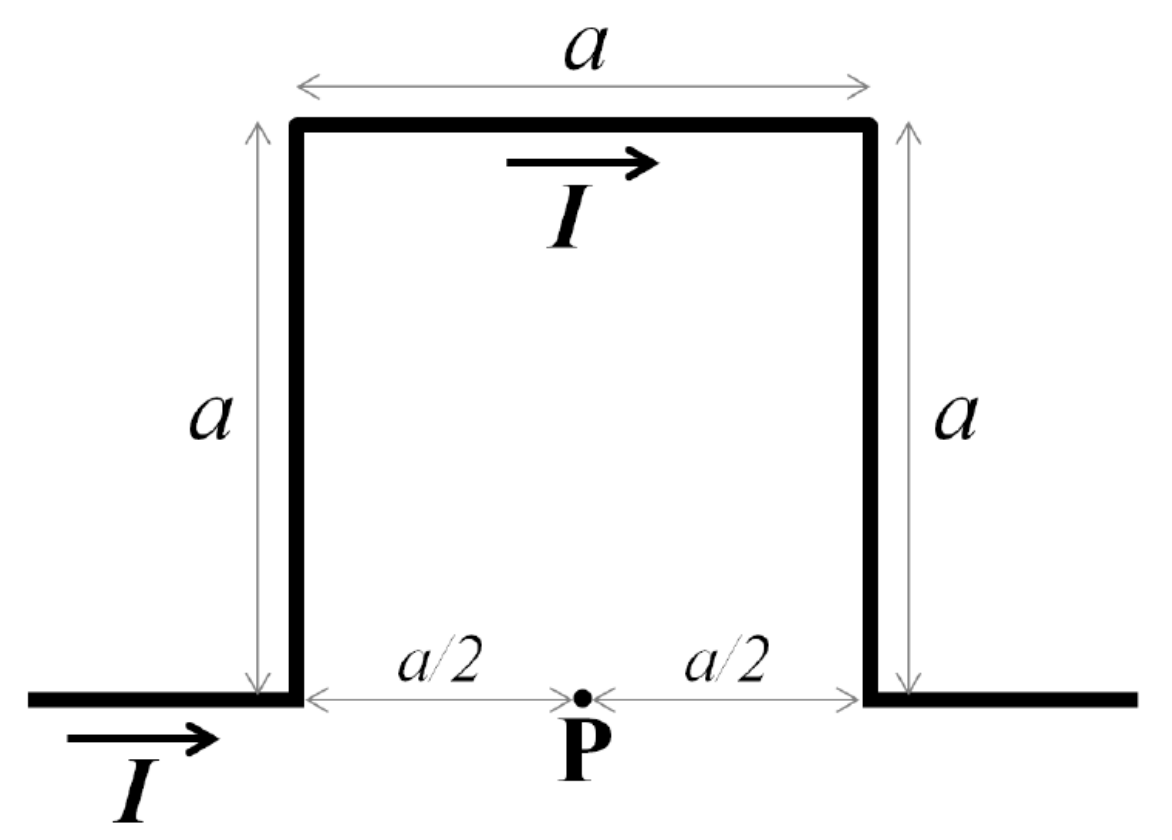
\includegraphics[width=4cm]{oz04/resources/oef-2-opgave.png}
    
%     \textbf{Figuur 4.2}
% \end{figure}

% \begin{description}[labelwidth=1.5cm, leftmargin=!]
%     \item[Geg. :]   $ \vec{I} $; $ a $;
% \end{description}

% \begin{figure}[H]
%     \centering
%     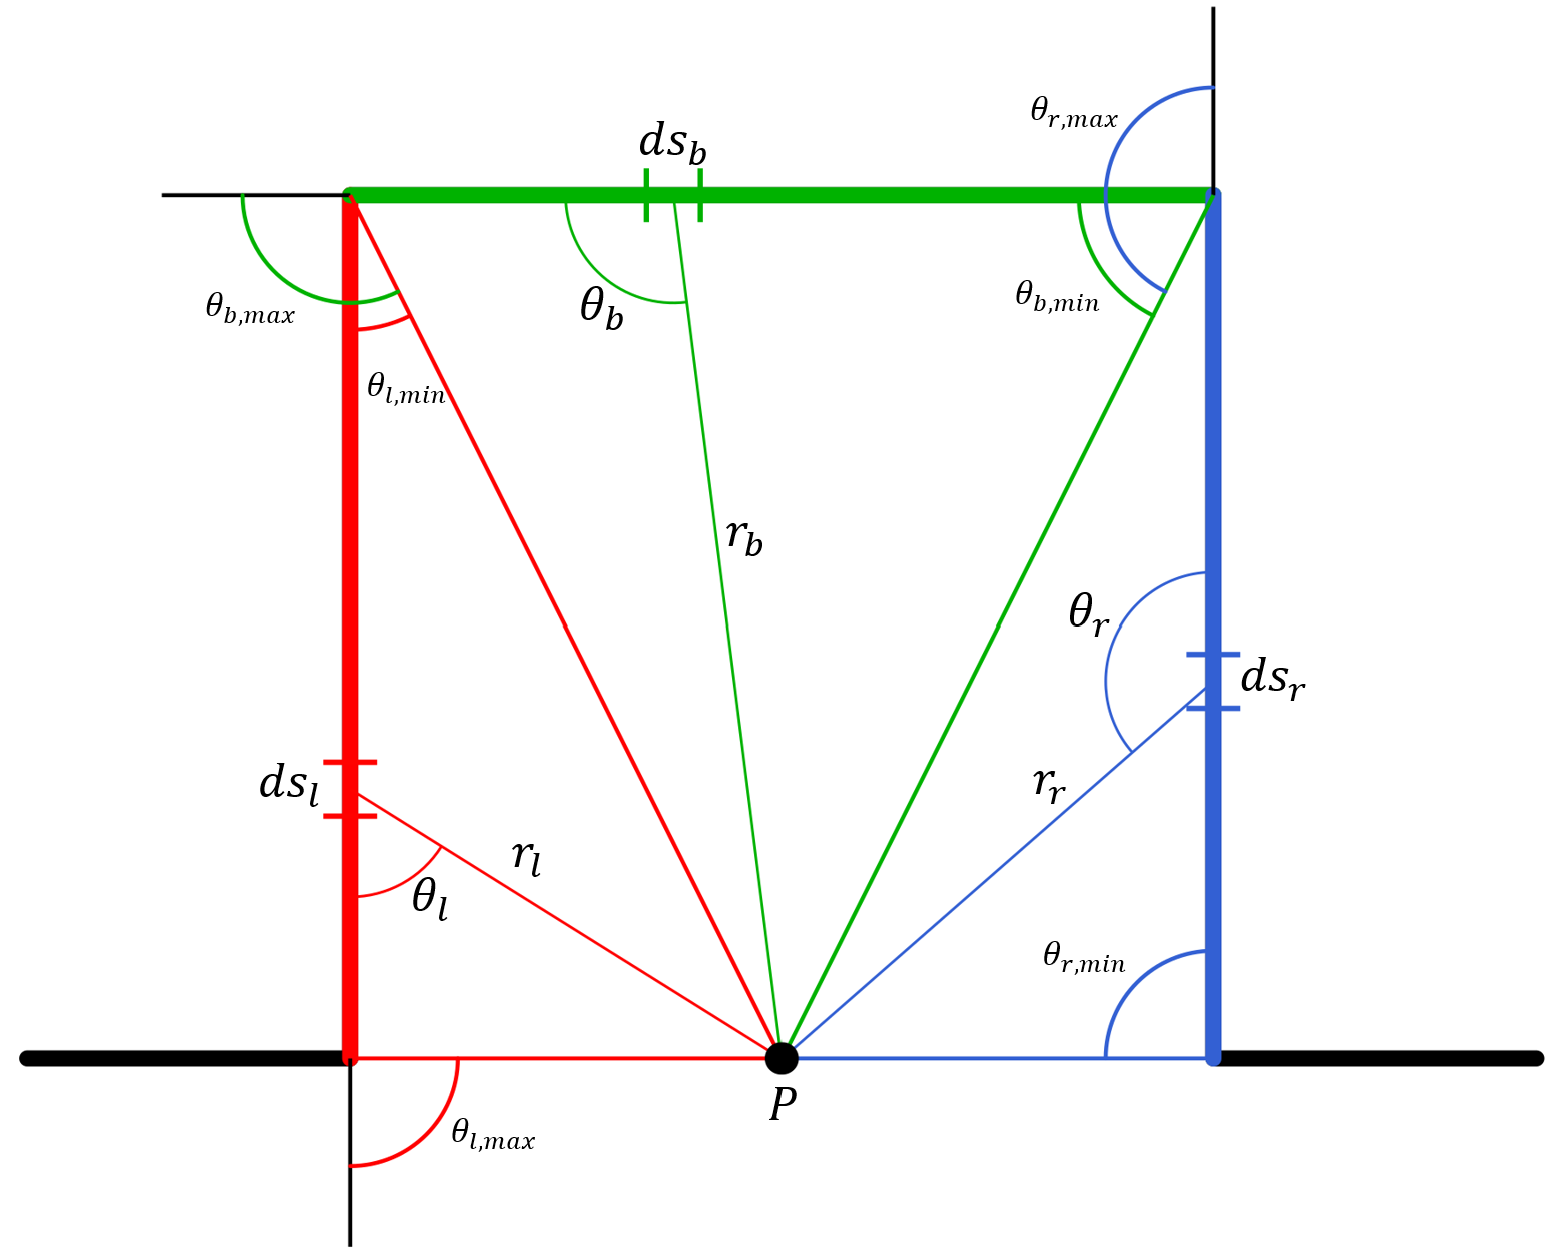
\includegraphics[width=8cm]{oz04/resources/oef-2-schets.png}
    
%     \textbf{Schets 4.1}
% \end{figure}

% \begin{description}[labelwidth=1.5cm, leftmargin=!]
%     \item[Gevr. :]  $ \vec{B} $;
%     \item[Opl. :]   $ \vec{B} = \vec{B}_{l} + \vec{B}_{b} + \vec{B}_{r} $
    
%                     Bekijk voorbeeld 28.11 in de slides voor uitleg bij berekeningen.
    
%                     $ d\vec{B}_{l} = -k_m \dfrac{I d\vec{s}_l \times \hat{r}_l}{r_l^2} $
                    
%                     \hspace{0.35cm} $ 
%                     = -k_m \dfrac{I ds_l \sin{\theta_l} \hat{k}}{r_l^2} $
                    
%                     \hspace{0.35cm} $ 
%                     = -k_m \dfrac{I ds_l \sin{\theta_l} \hat{k}}{\left( \dfrac{a}{2 \sin{\theta_l}} \right)^2} $
                    
%                     \hspace{0.35cm} $ 
%                     = -k_m \dfrac{I ds_l \sin^3{\theta_l} \hat{k}}{\left(\dfrac{a}{2} \right)^2} $
                    
%                     \begin{quote}
%                         \hspace{0.6cm} $ s_l = \dfrac{\dfrac{a}{2}}{\tan{\theta_l}} $
                        
%                         \hspace{0.05cm} $ \Rightarrow 
%                         \dfrac{d}{ds_l}\left( s_l \right) ds_l = \dfrac{a}{2} \dfrac{d}{d\theta_l}\left( \dfrac{1}{\tan{\theta_l}} \right) d\theta_l  $
                        
%                         \hspace{0.05cm} $ \Rightarrow 
%                         ds_l = \dfrac{a}{2} \cdot \left(- \dfrac{1}{\sin^2{\theta_l}} \right) d\theta_l $
%                     \end{quote}
                    
%                     \hspace{0.35cm} $ 
%                     = -k_m \dfrac{I \dfrac{a}{2} d\theta_l \sin{\theta_l} \hat{k}}{\left(\dfrac{a}{2} \right)^2} $
                    
%                     \hspace{0.35cm} $ 
%                     = -k_m \dfrac{2I \sin{\theta_l}}{a} d\theta_l \hat{k} $
                    
%                     \hspace{-0.57cm} $ \Leftrightarrow 
%                     \int_0^{\vec{B}_l}{d\vec{B}_l} = -k_m \dfrac{2I }{a} \hat{k} \int_{\theta_{l,min}}^{\theta_{l,max}}{\sin{\theta_l} d\theta_l} $
                    
%                     \hspace{-0.57cm} $ \Leftrightarrow 
%                     \vec{B}_l = -k_m \dfrac{2I}{a} \hat{k} (\cos{\theta_{l,max}} - \cos{\theta_{l,min}}) $
                    
%                     Gelijkaardige afleidingen voor $ \vec{B}_b $ en $ \vec{B}_r $ (Ga ik niet uitschrijven)
                    
%                     $ \vec{B}_b = -k_m \dfrac{I}{a} \hat{k} (\cos{\theta_{b,max}} - \cos{\theta_{b,min}}) $
                    
%                     $ \vec{B}_r = -k_m \dfrac{2I}{a} \hat{k} (\cos{\theta_{r,max}} - \cos{\theta_{r,min}}) $
                    
%                     \vspace{0.5cm}
                    
%                     $ \vec{B} = \vec{B}_{l} + \vec{B}_{b} + \vec{B}_{r} $
                    
%                     \hspace{0.3cm} $ 
%                     = -k_m \dfrac{I}{a} \hat{k} \left( 2 \left( \cos{\theta_{l,max}} - \cos{\theta_{l,min}} \right) + \left( \cos{\theta_{b,max}} - \cos{\theta_{b,min}} \right) + 2 \left( \cos{\theta_{r,max}} - \cos{\theta_{r,min}} \right) \right) $
                    
%                     \hspace{0.3cm} $ 
%                     = -k_m \dfrac{I}{a} \hat{k} \left( 2 \left( \cos{90^{\circ}} - \cos{\left( \arctan{\dfrac{1}{2}} \right) } \right) + \left( \cos{\left( 90^{\circ} + \arctan{\dfrac{1}{2}} \right)} - \cos{\left( \arctan{2} \right) } \right) + 2 \left( \cos{\left( 90^{\circ} + \arctan{2} \right) } - \cos{90^{\circ}} \right) \right) $
                    
%                     \hspace{0.3cm} $ 
%                     = -k_m \dfrac{I}{a} \hat{k} \cdot 2\sqrt{5} $
                    
%                     \hspace{0.3cm} $ 
%                     = -\dfrac{\mu_0}{4\pi} \dfrac{I}{a} \hat{k} \cdot 2\sqrt{5} $
                    
%                     \hspace{0.3cm} $ 
%                     = -\dfrac{\sqrt{5} \mu_0 I}{2 \pi a} \hat{k} $
% \end{description}

% \vspace{1cm}